\documentclass[a4paper,10pt]{article}
\usepackage[utf8]{inputenc}
\usepackage{datetime}
\usepackage{listings}
\usepackage{graphicx}
\newdate{date}{17}{03}{2017}
\date{\displaydate{date}}

\title{Homework 3\\Marlen Akimaliev\\BIL622-Numerical Analysis II}
%\author{Share\LaTeX}

\begin{document}

\maketitle

\section{Problem}
Given the second order differential equation $(x^2+1)\times y'' = 2 \times x \times y'$ with initial conditions $y(0)=1, y'(0)=3$ at the interval $[0;1]$, find the solution using Runge-Kutta $4^{th}$ order method with $h=0.2$. Compare results with the solution of the equation given by $y = -x^3+3 \times x +1$.
\section{Solution}
It works by splitting the problem into 2 first-order differential equations:\\
$y'=u$\\
$u'=f(x,y,u)$\\
In our case it will be as follows:\\
Equations is given as: $(x^2+1)y"-2xy'=0; y(0)=1;y'(0)=3$\\
Splitting into 2:\\
$y"=2xy'/(x^2+1)$ or the $f(x,y,y')$\\
$u'=2xu/(x^2+1)$ or the $f(x,y,u)$\\
Solution for 6 points as a table in the interval $[0, 0.5]$ is as follows:
\begin{center}
\begin{tabular}{ |c|c| } 
 \hline
 $x$ & $y$\\
\hline
 $0.0$ & $1.0000000000000000$\\
 $0.2$ & $1.6079992157631604$\\
 $0.4$ & $2.2639946460128000$\\
 $0.6$ & $3.0159859627546286$\\
 $0.8$ & $3.9119736243068348$\\
 $1.0$ & $4.9999579899703832$\\
 \hline
\end{tabular}
\end{center}
We can use the following expression to evaluate the absolute error, which is the sum of the absolute values of the residuals:\\
$$\varepsilon_{abs} = \sum_{i=1}^{N} |y(x_i)-w_i|$$\\
I have used the following Python code \cite{klopper} to evaluate values and plot the graph.
\begin{lstlisting}[language=Python]
from matplotlib import pyplot as plt
import numpy as np

x = 0.0
y = 1.0
u = 3.0

h = 0.2
vx=[]
vy=[]

print "x   ", "y"
print("%4.1f %10.16f" % (x, y))

while(x<1.0):
	m1 = u
	k1 = 2*x*u/(x**2+1)
	m2 = u + (h/2.)*k1
	x_2 = x + (h/2.)
	y_2 = y + (h/2.)+m1
	u_2 = m2
	k2 = 2*x_2*u_2/(x_2**2+1)
	m3 = u + (h/2.)*k2
	x_3 = x + (h/2.)
	y_3 = y + (h/2.) * m2
	u_3 = m3
	k3 = 2*x_3*u_3/(x_3**2+1)
	m4 = u + h * k3
	x_4 = x+h
	y_4 = x+h*m3
	u_4 = m4
	k4 = 2*x_4*u_4/(x_4**2+1)
	x = x + h
	y = y + (h/6.)*(m1+(2.*m2)+(2.*m3) + m4)
	u = u + (h/6.)*(k1+(2.*k2)+(2.*k3) + k4)
	vx.append(x)
	vy.append(y)

def y(x):
	return -x**3+3*x+1

yx = []
for v in vx:
	yx.append(y(v))

def error_abs(v,w):
	total_err = 0
	for i in range(0,len(v)):
		total_err = total_err + np.abs(v[i]-w[i]) 
	return total_err

for x, y in list(zip(vx, vy))[::1]:
    print("%4.1f %10.16f" % (x, y))
plt.plot(vx, vy, label='approximation' )
plt.plot( vx, yx, linestyle='--',label='exact' )
plt.title( "Approximate solution of equation with Runge-Kutta method 4")
plt.xlabel('Value of x') 
plt.ylabel('Value of y')
plt.legend(loc=4)
plt.grid()
plt.savefig( '1_1.eps', fmt='EPS', dpi=100 )
plt.show()

err = error_abs(yx, vy)
print err
\end{lstlisting}
Error value equals to $3.59991143881$.\\
If we try to plot these values and the exact function as a graph result is as follows:
\begin{figure}[ht]
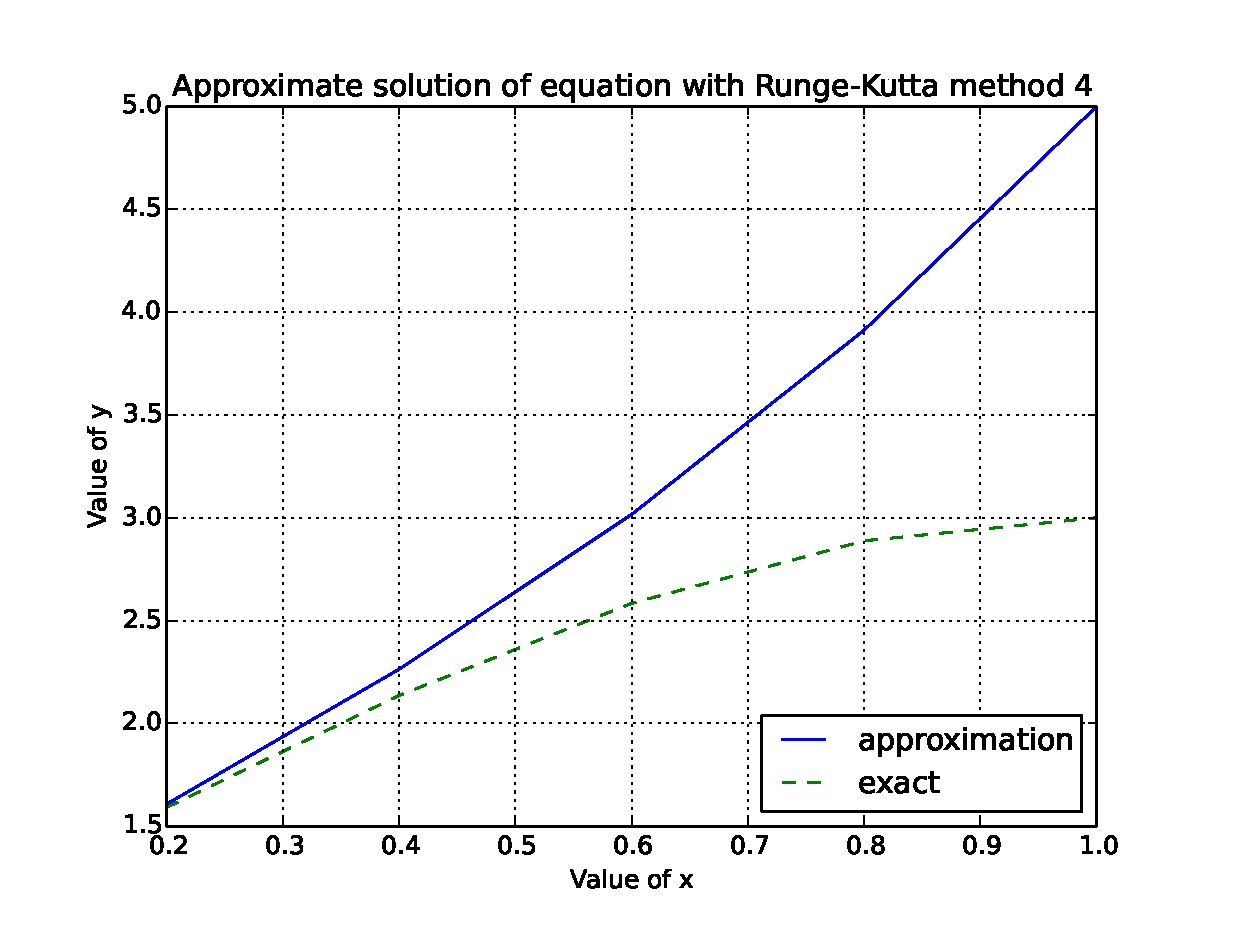
\includegraphics[width=8cm]{1_1.eps}
\end{figure}

\medskip

\begin{thebibliography}{9}
\bibitem{klopper} Second order ODE solved with RK4 in Python, \\\texttt{https://www.youtube.com/watch?v=-k64Xa0onfQ}
\end{thebibliography}

\end{document}
